\chapter{System Design}
\label{chp:system_design}
% In this section, we will present the design of our framework that transforms a standard single-device CNN into a communication-efficient distributed execution tasks across a cluster of networked MCUs. We will first discuss the overall architecture of coordinator-worker model, followed by the communication protocols. Two core optimizations techniques, i.e., \emph{block-wise local execution} and \emph{cross-block data reuse}, are proposed to allieviate the communication overhead, and will be discussed in detail. \textcolor{red}{We analyze the conditions for our proposed optimizations.} 
%% and provide a cost model to evaluate the trade-offs between communication and computation. Finally, we will discuss the implementation details of our framework.

In this chapter, we present the design of our framework that transforms a standard single-device CNN into a set of communication-efficient distributed execution tasks across a cluster of networked MCUs. We first describe the overall coordinator-worker architecture and a two-stage execution pipeline. Then, we detail the offline preprocessing stage, which quantizes the CNN model and compiles it into an execution plan in JSON format (Section~\ref{sec:offline-preprocessing}), and the online inference stage, which carries out the plan over a lightweight application protocol in TCP/IP (Section~\ref{sec:online-inference}). On top of this runtime inference, we develop two core optimization techniques that alleviate the communication and memory overhead of the system: \emph{block-wise local execution} (Section~\ref{sec:block-wise-local-execution}) and \emph{cross-block data reuse} (Section~\ref{sec:cross-block-data-reuse}). Between these two optimizations, we introduce an \emph{overlap-ratio cost model} (Section~\ref{sec:overlap-ratio-cost-model}) that characterizes when block-wise local execution stops paying off, and for cross-block data reuse we analyze the conditions under which it preserves correctness and improves performance (Section~\ref{sec:cross-conditions}). 

\section{System Architecture}
\label{sec:system-architecture}

\begin{figure}[t]
    \center
    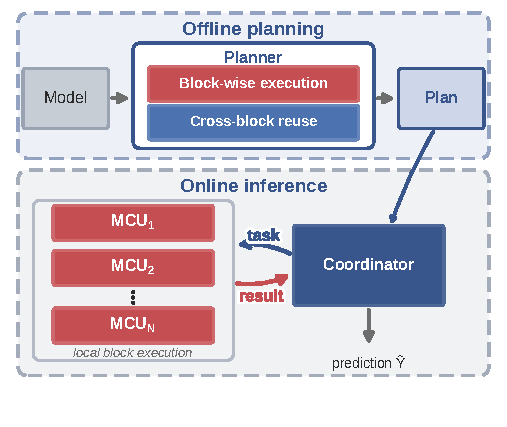
\includegraphics[width=\textwidth,height=0.3\textheight,keepaspectratio]{figs/fig_overview.pdf}
    \caption{Overview of our system architecture, comprising an offline preprocessing stage that compiles the model into an execution plan and per-worker manifests, and an online stage that executes the plan on a coordinator-worker cluster.}
    % \vspace{-4mm}
    \label{fig:system-architecture}
\end{figure}

As discussed in Section~\ref{chp:system_design}, a typical MCU offers only hundreds of KBs of SRAM (e.g., less than 512~KB) during runtime inference. \textcolor{red}{While the model weights can be stored in Flash memory, the intermediate activations must reside in SRAM at runtime. For CNNs built from IRBs, the largest tensor at runtime is the output of the expanding convolution layer: each block first expands the channel dimension by an expansion ratio $e$ (e.g., $e=6$ in MobileNetV2), applies a depthwise convolution, and then reduces the channel dimension back to the original size (refs).} The output of the expanding convolution layer is therefore $e$ times larger than the input, which can easily exceed the SRAM capacity of a single MCU. This results in a significant memory bottleneck that prevents the execution of large CNNs on resource-constrained MCUs. 

To address this, we implement an end-to-end pipeline for distributed inference across multiple networked MCUs, as shown in Figure~\ref{fig:system-architecture}, comprising two stages:
\begin{itemize}
    \item \textbf{Offline preprocessing stage}: It performs an 8-bit quantization of the model, and extracts the metadata describing the model weights and structural information. The metadata is emitted as JSON files and serialized into the Flash memory of each MCU at compilation time. An \emph{execution plan} is generated that describes the inference strategy and the data flow between the MCUs.
    
    \item \textbf{Online inference stage}: It executes the model on the distributed system across multiple networked MCUs. A single \emph{coordinator} holds the model metadata and the execution plan, partitions the workload to the \emph{workers} at each step, and reassembles the workers' outputs to produce the final inference result. Each \emph{worker} stores its share of the weights and activations, and performs the assigned computation tasks. The coordinator and workers communicate through a lightweight protocol on top of TCP/IP.
\end{itemize}

% As discussed in Section~\ref{chp:system_design}, a typical MCU offers only hundreds of KBs of SRAM (e.g., less than 512~KB) during runtime inference. While the model weights could be stored in the Flash memory, the intermediate activations have to reside in the SRAM at runtime, resulting in a significant memory bottleneck. 

% To address the issue, we implement a end-to-end pipeline shown in Figure~\ref{fig:tbd} that incorporates:
% \begin{itemize}
%     \item \textbf{Offline preprocessing stage} that quantizes the model, and extracts the metadata for the model weights and intermediate activations. The metadata will be released as JSON files and serialized into the Flash memory of each MCU at compilation time. An \emph{execution plan} will be generated to describe inference strategy and the data flow between the MCUs. 
    
%     \item \textbf{Online inference stage} that executes the model in the distributed system across multiple networked MCUs. A single \emph{coordinator} holds the model metadata and the execution plan, partitions the workload to the \emph{workers} at each step, and reassables the workers' outputs to produce the final inference result. Each \emph{worker} stores its share of the weights and activations and performs the assigned computation tasks. The coordinator and workers communicate through a lightweight protocol under TCP/IP. 
% \end{itemize}

\section{Offline Preprocessing}
\label{sec:offline-preprocessing}


\subsection{Quantization}

\subsection{Planner}


\section{Online Inference}
\label{sec:online-inference}
The coordinator-worker architecture is designed to execute the distributed inference tasks efficiently. As demonstrated in Figure~\ref{fig:tbd}, a coordinator is responsbile for the task scheduling and data aggregation. Based on the execution plan, the coordinator partitions the input activations, wraps and assigns the computation tasks to workers, and gather results from workers to produce the output activations. Each worker is in charge of executing the assigned tasks, which includes loading model weights in Flash, selecting the suitable computation kernel, and performing the computation on the input activations.

\subsection{Coordinator Design}

\subsection{Worker Design}

\subsection{Protocol Design}




\section{Block-wise Local Execution}
\label{sec:block-wise-local-execution}
To optimize performance and resource utilization, we have implemented a block-wise local execution strategy. This approach allows us to process data in smaller chunks, reducing memory overhead and improving execution speed. Each block is processed independently, allowing for parallel execution and better load balancing across the system. This design choice also enhances fault tolerance, as failures in one block do not affect the processing of others.

\section{Overlap-ratio Cost Model}
\label{sec:overlap-ratio-cost-model}
We have implemented a hybrid scheduling mechanism that combines the benefits of both centralized and decentralized approaches. This allows for more efficient resource allocation and load balancing across the system.

\section{Cross-block Data Reuse}
\label{sec:cross-block-data-reuse}
To further optimize performance, we have implemented a cross-block data reuse mechanism. This allows data generated in one block to be efficiently utilized in subsequent blocks, reducing redundant computations and improving overall system efficiency.

\section{Conditions to Enable Cross-block Data Reuse}
\label{sec:cross-conditions}
Some conditions for cross-block data reuse include:
\begin{itemize}
    \item Data must be compatible across blocks.
    \item The data must be stored in a format that allows for easy retrieval and reuse.
    \item The system must ensure that the reused data is up-to-date and valid for the current block's processing requirements.
\end{itemize}




